\begin{center}
    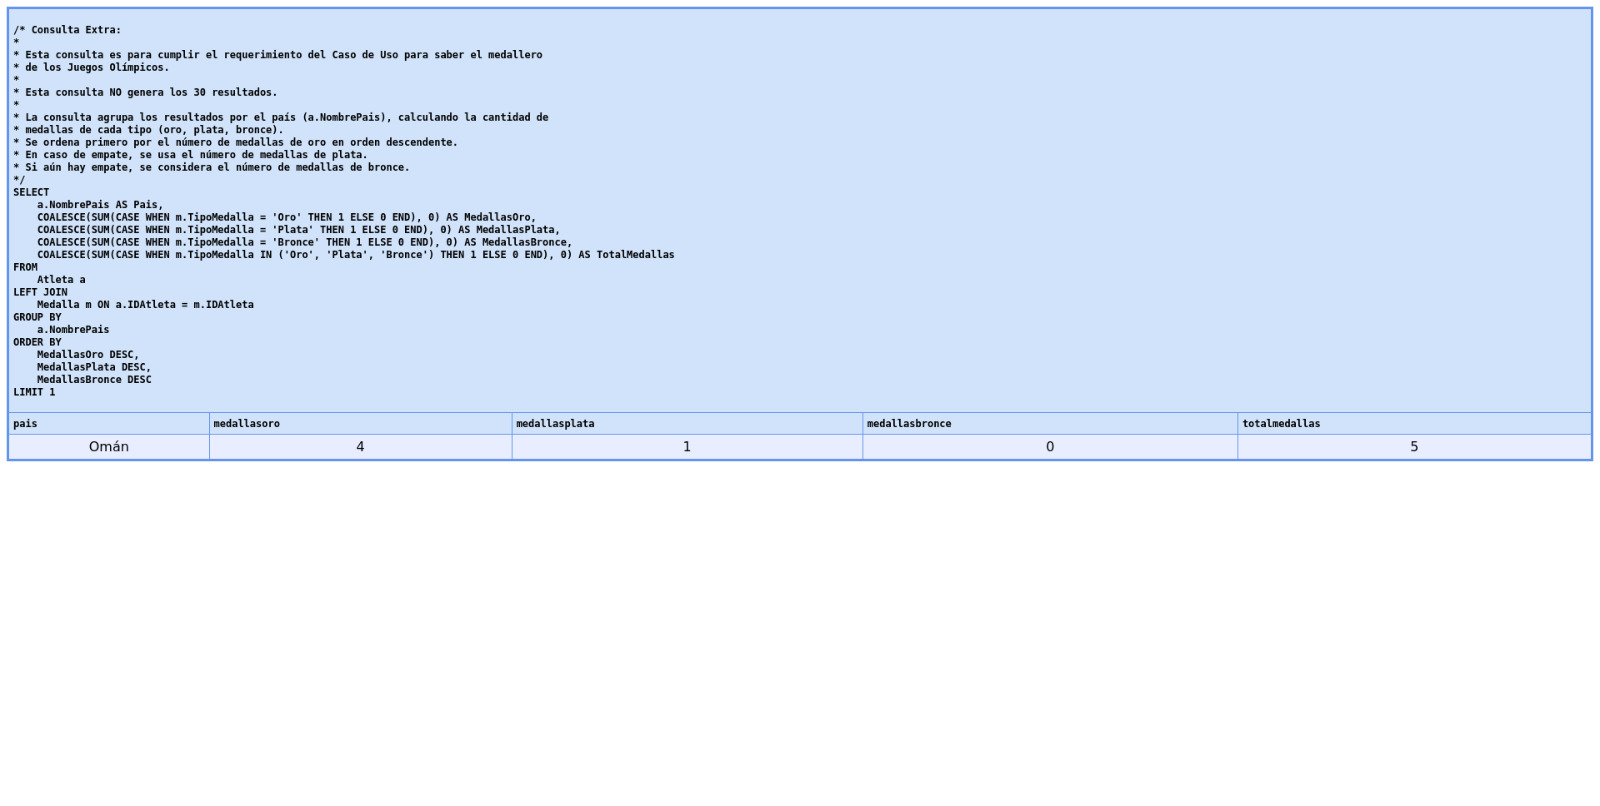
\includegraphics[width=16.5cm]{resources/ConsultaExtra.jpeg} 
    
   Consulta Extra. Medallero de los Juegos Olímpicos.
\end{center}

\textbf{Propósito de la consulta}

El objetivo de esta consulta es generar el medallero de los Juegos Olímpicos, mostrando la cantidad de medallas de oro, plata y bronce obtenidas por cada país, con un orden que prioriza el número de medallas de oro, seguido por las de plata y bronce.

\textbf{Desglose de la consulta}

\begin{itemize}
   \item \textbf{Selección de columnas (\texttt{SELECT})}:
   \begin{itemize}
       \item \texttt{a.NombrePais}: Nombre del país que será representado en el medallero.
       \item \texttt{COALESCE(SUM(CASE ...))}: Suma la cantidad de medallas de cada tipo (oro, plata, bronce), reemplazando valores nulos con 0.
       \item \texttt{TotalMedallas}: Suma total de medallas (oro, plata y bronce) obtenidas por el país.
   \end{itemize}

   \item \textbf{Tablas involucradas (\texttt{FROM} y \texttt{JOIN})}:
   \begin{itemize}
       \item \texttt{Atleta (a)}: Contiene información sobre los atletas y su país de origen.
       \item \texttt{Medalla (m)}: Contiene información sobre las medallas obtenidas por los atletas.
       \item Se utiliza un \texttt{LEFT JOIN} entre \texttt{Atleta} y \texttt{Medalla} para incluir a los países incluso si no tienen medallas registradas.
   \end{itemize}

   \item \textbf{Agrupación de resultados (\texttt{GROUP BY})}:
   \begin{itemize}
       \item Los resultados se agrupan por \texttt{a.NombrePais}, asegurando que cada país tenga un único registro con el conteo de sus medallas.
   \end{itemize}

   \item \textbf{Ordenamiento de resultados (\texttt{ORDER BY})}:
   \begin{itemize}
       \item Los resultados se ordenan jerárquicamente:
       \begin{enumerate}
           \item Por \texttt{MedallasOro} en orden descendente.
           \item En caso de empate, por \texttt{MedallasPlata}.
           \item En caso de persistir el empate, por \texttt{MedallasBronce}.
       \end{enumerate}
   \end{itemize}

   \item \textbf{Límite de resultados (\texttt{LIMIT 1})}:
   \begin{itemize}
       \item La consulta devuelve solo el país con más medallas de oro (y desempates por plata y bronce), ya que está limitada a un solo resultado.
   \end{itemize}
\end{itemize}

\textbf{Análisis detallado}

\begin{enumerate}
   \item \textbf{Relación entre tablas:}
   \begin{itemize}
       \item La consulta vincula a los atletas con las medallas que han ganado utilizando \texttt{a.IDAtleta = m.IDAtleta}.
       \item El \texttt{LEFT JOIN} asegura que los países sin medallas aún se incluyan en la lista, aunque con valores de medallas igual a cero.
   \end{itemize}

   \item \textbf{Cálculo de medallas:}
   \begin{itemize}
       \item Las expresiones \texttt{CASE WHEN} cuentan medallas específicas (oro, plata, bronce), sumando los valores que corresponden.
       \item \texttt{COALESCE} reemplaza valores nulos con 0, útil para países que no tienen medallas de cierto tipo.
   \end{itemize}

   \item \textbf{Orden y desempate:}
   \begin{itemize}
       \item El orden por tipos de medallas asegura que los países con mejor desempeño sean priorizados correctamente.
   \end{itemize}
\end{enumerate}

\textbf{Consideraciones}

\begin{itemize}
   \item \textbf{Países sin medallas:}
   \begin{itemize}
       \item Gracias al \texttt{LEFT JOIN}, los países sin medallas no son excluidos, pero tendrán valores de medallas igual a cero.
   \end{itemize}
   \item \textbf{Empates:}
   \begin{itemize}
       \item Si dos países tienen exactamente el mismo número de medallas de oro, plata y bronce, el orden relativo entre ellos no está definido.
   \end{itemize}
\end{itemize}

\textbf{Utilidad de la consulta}

Esta consulta permite:
\begin{itemize}
    \item Generar estadísticas sobre el rendimiento de cada país en los Juegos Olímpicos.
    \item Identificar rápidamente el país más exitoso basado en el conteo de medallas.
    \item Evaluar tendencias en el desempeño de países durante la competencia.
\end{itemize}

\textbf{Nota sobre el \texttt{LIMIT 1}}

Si se elimina la cláusula \texttt{LIMIT 1}, la consulta generará el medallero completo, mostrando los resultados para todos los países en orden de prioridad basado en el número de medallas de oro, plata y bronce.
